În cele ce urmează voi prezenta soluția software propusă pentru managementul bazelor de date în maniera descrisă anterior. Voi trece în revistă arhitectura software, urmând apoi să explic fiecare din componentele aplicației, precum și modul de interacționare a acestora.
\\

\section{Arhitectura sistemului software}
Sistemul este împărtit în 3 componente importante:
\begin{itemize}
\item Scripturi UNIX ce interacționează cu instanțele de baze de date;
\item RESTful API folosit pentru a expune funcționalitatea oferită de scripturi prin intermediul protocolului HTTP;
\item Aplicație Web ce comunică prin intermediul protocolului HTTP cu API-ul RESTful expus.
\end{itemize}
În \textit{Figura 2} este prezentată diagrama arhitecturii software.
\begin{figure}[h]
	\centering
	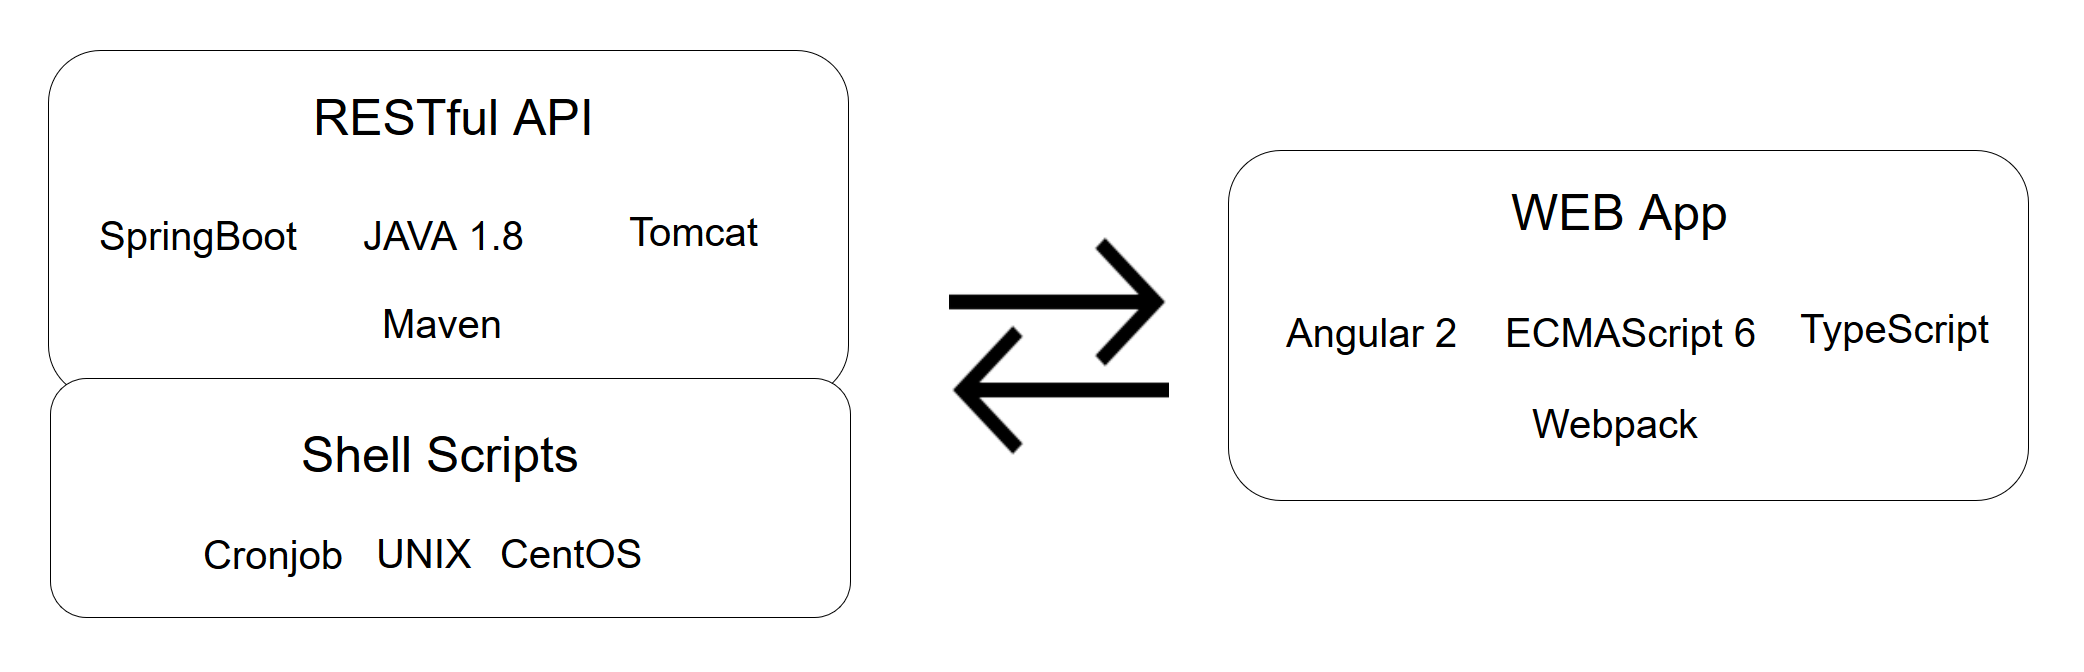
\includegraphics[scale=0.30]{LayeredArchLandscape}
    \caption{Diagrama arhitecturii software}
    \label{fig:LayeredArchPortrait}
\end{figure}
\newpage
\section{Scripturile UNIX}
Funcționalitatea de bază a aplicației constă în interacționarea cu instanțele de baze de date. Pentru asta am făcut 3 scripturi ce au urmatoarele responsabilități:
\begin{enumerate}
\item \textbf{pg-script.sh} pentru interacționarea cu instanțele (pornire, oprire, interogare status);
\\
\begin{listing}[ht]
\inputminted[
frame=lines,
framesep=2mm,
baselinestretch=0.9,
fontsize=\footnotesize,
fontfamily=courier,
linenos
]{bash}{sourceCode/pg-script.sh}
\caption{\texttt{pg-script.sh}}
\label{cod:pgScript} 
\end{listing}
\item \textbf{basebackup.sh} pentru crearea de basebackup a unei instanțe (checkpoint de la care să se poate începe procesul de restaurare);
\\
\begin{listing}[ht]
\inputminted[
frame=lines,
framesep=2mm,
baselinestretch=0.9,
fontsize=\footnotesize,
fontfamily=courier,
linenos
]{bash}{sourceCode/basebackup.sh}
\caption{\texttt{basebackup.sh}}
\label{cod:basebackup} 
\end{listing}
\item \textbf{recovery.sh} pentru inițierea procesului de restaurare a bazei de date
\\
\begin{listing}[ht]
\inputminted[
frame=lines,
framesep=2mm,
baselinestretch=0.9,
fontsize=\footnotesize,
fontfamily=courier,
linenos
]{bash}{sourceCode/recovery.sh}
\caption{\texttt{recovery.sh}}
\label{cod:recovery} 
\end{listing}
\end{enumerate}\
\par
Toate cele trei scripturi au fost gândite cu scopul de a se crea symbolic links (scurtături) către ele. Acestea vor avea numele insțantei bazei de date, iar scriptul principal folosește numele fișierului scurtatură pentru a accesa datele instanței respective. Scopul este acela de a crea un singur set de scripturi, iar dacă avem n instanțe de baza de date doar creem symbolic links către scripturi, fiecare cu numele instanței de baza de date respective.
\newpage
\section{Server-ul: RESTful API}
Pentru partea de server (backend) a fost aleasă soluția creării unui RESTful API cu scopul de a se expune funcționalitatea oferită de către scripturile bash prezentate anterior. Am utilizat Java Enterprise Edition, framework-ul Spring, ce faciltează crearea unui API prin intermediul librăriilor SpringWeb.
\par
Un alt motiv pentru care am ales Spring a fost suportul oferit pentru a injecta dependințe urmând șablonul de proiectare Dependency Injection. Astfel, am decuplat controller-ul REST ce primește cererea web de către serviciul care o execută. Se poate injecta orice implementare de serviciu în controller, iar codul acestuia nu trebuie schimbat. Versiunea de Java utilizată este 1.8.
\begin{listing}[ht]
\inputminted[
frame=lines,
framesep=2mm,
baselinestretch=0.9,
fontsize=\footnotesize,
fontfamily=courier,
linenos
]{java}{sourceCode/DatabaseManagementAPI.java}
\caption{\texttt{DatabaseManagementAPI.java}}
\label{cod:DatabaseManagementAPI} 
\end{listing}
\newpage
Pentru managementul dependințelor și crearea artefactului s-a folosit Maven. Se oferă ca și exemplu fișierul \textbf{pom.xml}:
\begin{listing}[ht]
\inputminted[
frame=lines,
framesep=2mm,
baselinestretch=0.9,
fontsize=\footnotesize,
fontfamily=courier,
linenos
]{xml}{sourceCode/pom.xml}
\caption{\texttt{pom.xml}}
\label{cod:pom} 
\end{listing}

\newpage
\section{Interfața grafică cu utilizatorul}
Scopul proiectului este crearea unei aplicații care să faciliteze manipularea serverelor de baze de date PostgreSQL de către dezvoltatori care nu trebuie să aibă acces la mașinile pe care se află bazele de date/ cunoștinte de UNIX. În acest sens, având deja server-ul de Java care expune prin servicii Web funcționalitățile respective, trebuie apelate și oferite într-o manieră cât mai intuitivă. 
\par
Ca și framework am folosit Angular 2, limbajul de programare fiind Javascript, standardul ECMAScript6, împreună cu TypeScript. Angular 2 are urmatoarele avantaje:
\begin{itemize}
\item este un framework open-source JavaScript construit și întreținut de Google, ceea ce usurează dezvoltarea aplicațiilor web.
\item standardizează aplicațiile la nivel de client (browser), oferind o structură robustă și ușor de implementat în dezvoltarea site-urilor.
\item este alegerea potrivită pentru orice aplicație web, în special dacă se preferă efectele vizuale spectaculoase. Rezultatul este un site fluid și rapid. Acesta este motivul pentru care se pretează SPA-urilor (Single Page Application) și aplicațiilor web destinate dispozitivelor mobile.
\item se integrează ușor cu Bootstrap, permite crearea de aplicații responsive care pot fi accesate atât din browserul calculatorului cât și de pe dispozitivele mobile. Astfel, este ușor să creezi o singură aplicație web care să se vadă perfect pe orice dispozitiv de pe care este accesată – PC, tabletă, telefon, plasmă.
\end{itemize}
\par Ca și manager de pachete am utilizat \textbf{npm} de la NodeJS.
\newpage
\section{Setarea aplicației în Amazon Web Services}
Având ca și obiectiv crearea unui mediu cât mai apropiat de cel aflat pe mașinile din producție, am închiriat un server EC2 de la Amazon.
\par
Sistemul de fișiere a fost stabilit conform descrierii din Capitolul 2. Am închiriat 3 discuri EBS(Elastic Block Storage) pe care le-am configurat precum a fost prezentat, pentru a seta 3 instanțe de baza de date.
\par 
Odată ce sistemul de fișiere a fost configurat, am creat scripturile ce vor interacționa cu bazele de date. Urmatorul pas a fost pornirea celor două servere (backend și frontend). În timpul acestui proces a fost necesară configurarea unui rol de securitate oferit mașinii de calcul EC2, pentru a permite traficul pe portul 3001 utilizat de aplicația frontend.